
\apendice{Documentación técnica de programación}

\section{Introducción}

En el siguiente anexo se describe la documentación técnica del programa, se detalla como está estructurado, cómo realizar la correcta instalación y configuración del mismo así como la batería de pruebas realizadas.

\section{Estructura de directorios}

\nombrePrograma se instala en la carpeta \textit{/usr/bin/} dentro un servidor Ubuntu. El programa consta de un script principal que mediante un daemon se ejecuta constantemente en segundo plano. Por cada ciclo de ejecución (por defecto es de un minuto) se descargan los datos en bruto desde PRTG que se almacenan en la carpeta \textit{/usr/bin/Monitorizacion\_IOT/Gestion\_Data/Logs/}. De ahí son procesados y guardados temporalmente en la carpeta

\textit{/usr/bin/Monitorizacion\_IOT/Gestion\_Data/TempData\_sensores/} 

Al realizar el entrenamiento o la predicción de los sensores se cargan los modelos de dichos sensores, estos se encuentran almacenados en \textit{/usr/bin/Monitorizacion\_IOT/Prediccion/modelos/}

En la carpeta \textit{/usr/bin/Monitorizacion\_IOT/Utilidades/} se encuentran diversas funciones de utilidad. 

\begin{figure}[h]
	\dirtree{%
		.1 /.
		.2 usr.
		.3 bin.
		.4 Monitorizacion\_IOT.
		.5 Gestion\_datos.
		.7 Load.
		.7 Logs.
		.7 TempData\_sensores.
		.5 Prediccion.
		.7 modelos.
		.5 Utilidades.
	}
	\caption{Directorios del proyecto}
	\label{directoriosdelproyecto}
\end{figure}

\newpage
\section{Manual del programador}

El manual del programador tiene como objetivo ayudar a todas aquellas personas que vayan a trabajar en este proyecto.
\subsection{Entorno de desarrollo}

Para la realización de este proyecto se necesita tener instalados los siguientes programas y dependencias:

\begin{itemize}
    \item Python 3: versión 3.8.10 
    \item Elasticsearch: versión 7.4
    \item kibana: versión 7.14.1
    \item logstash: versión 7.14.1
    \item openjdk-11-jre-headless: versión 11.0.11
\end{itemize}
Librerías python:
\begin{itemize}
    \item river versión 0.71
    \item pandas: versión 1.3.2
    \item Elasticsearch: versión 7.14.0
    \item numpy: versión 1.21.2
\end{itemize}

\subsubsection{Archivos}

\begin{itemize}
    \item \textbf{Monitorizacion\_IOT.sh}: Este es el script principal de la aplicación el cual esta hilado a un daemon, de tal forma que se repite en bucle cada minuto en el cual se descargan los datos de PRTG, se suben a Elasticsearch, se realiza el entrenamiento y la predicción de cada sensor.
    
    \item \textbf{/Gestion\_datos/Descargar\_data.sh}: Es el script que se encarga de descargar los datos de PRTG, transformar dichos datos y subirlos a Elasticsearch
    
    \item \textbf{/Gestion\_datos/Borrar\_datos\_predicciones.sh}: Debido a que para cada sensor se repite la predicción cada minuto y se suben los resultados a Elasticsearch es necesario borrar la predicción anterior para que siempre se pueda visualizar la predicción actualizada, este script hace exactamente eso.
    
    \item \textbf{/Gestion\_datos/Load\_sensor\_data.sh}: Este script se encarga de enviar línea por línea de un fichero a logstash para poder ser enviado a Elasticsearch
    
    \item \textbf{/Predicciones/Crear\_modelo.py}: En este fichero el usuario puede configurar y crear un modelo para un sensor.
    
    \item \textbf{/Predicciones/Modelo.py}: En este fichero se encuentran las clases que corresponden a todos los modelos.
    
    \item \textbf{/Predicciones/Persistencia\_modelo.py}: En este fichero se encuentra la clase que permite guardar en disco y cargar cada modelo
    
    \item \textbf{/Predicciones/Realizar\_entrenamiento.py}: Es el fichero encargado de la realización del entrenamiento del modelo de un sensor, se carga el modelo correspondiente al sensor, se descargan los últimos datos subidos a Elasticsearch y se realiza en entrenamiento del modelo, se suben las predicciones realizadas durante el entrenamiento por el modelo a Elasticsearch y finalmente se guarda el modelo en disco.
    
    \item \textbf{/Predicciones/Realizar\_prediccion.py}: Es el fichero encargado de realizar la perdición de un sensor, se carga el modelo correspondiente al sensor que se desea predecir y se realza la perdición a partir de la fecha actual y tantos instantes de tiempo cómo este especificado en el fichero principal, Monitorizacion\_IOT.sh.
    
    \item \textbf{/Utilidades/campos.py}: En este fichero se encuentra una clase de enumeración donde se encuentran los tres tipos de campos que se suben a Elasticsearch.
    \begin{itemize}
        \item \textbf{VALOR}: Corresponde al valor real recogido por el sensor.

        \item \textbf{PREDICCION}: Corresponde al valor de la predicción 
        \item \textbf{ENTRENAMIENTO}:Corresponde al valor del entrenamiento.
    \end{itemize}
    
    \item \textbf{/Utilidades/Extractor.py}: En este fichero se encuentra la clase encargada de la descarga de datos de Elasticsearch.
    
    \item \textbf{/Utilidades/Generador\_lineas.py}: En este fichero se encuentra la clase encargada de generar las líneas de texto en un formato específico para poder ser procesadas por logstash. 
    
    \item \textbf{/Utilidades/Tatamiento\_sensor\_data.py}: En este fichero se encuentra la clase encargada de tratar con los datos de los sensores, permite leer ficheros JSON y transformarlos.
    
    \item \textbf{/Utilidades/Transformar\_data.py}: Es el fichero encargado de transformar los ficheros JSON con los datos procedentes de PRTG en un fichero apto para ser procesado por Logstash. 
    
\end{itemize}

\begin{comment}
\subsection{Mover ficheros al servidor}
En este apartado se mostrará una forma en la que se pueden mover ficheros entre un servidor ubuntu y el host.

c:\pscp elk@192.168.0.29:MonitorzacionIOT\_1.0\_all.deb .

c:\pscp "C:\Users\mella\Documents\MonitorzacionIOT\_1.0\_all.deb"

pi@192.168.0.31:MonitorzacionIOT\_1.0\_all.deb
\end{comment}

\subsection{Implementar nuevos modelos}

\nombrePrograma es flexible a la implementación de nuevos modelos de incremental learning, para crear un nuevo modelo se ha de acceder a la carpeta donde se ha instalado el programa y editar el fichero \textit{/Predicciones/Modelo.py}, en este fichero se puede ver la clase abstracta \textit{Modelo} la cual implementa cuatro métodos abstractos:
\begin{itemize}
    \item \textbf{inicializar(self)}: El método encargado de inicializar  el modelo, implementando el algoritmo deseado.
    
    \item \textbf{cargar(self, model)}:  El método encargado de cargar el modelo.
    
    \item \textbf{entrenar(self, datos)}: El método encargado del entrenamiento del modelo a partir de una serie de datos
    \item \textbf{predecir(self, horizonte)}: El método encargado de realizar la predicción a futuro de un sensor a partir de un modelo ya entrenado.
\end{itemize}

Para crear un nuevo modelo se a de programar una nueva clase que herede de \textit{Modelo} e implemente estas cuatro funciones.

\section{Compilación, instalación y ejecución del proyecto}

\subsection{Configuración Ubuntu Server}

Para albergar nuestro programa utilizaremos una máquina virtual Ubuntu Server.

Antes de comenzar la instalación tendremos que asegurarnos que estén instaladas las herramientas de red de Linux, las cuales ayudarán a saber la IP, y con ella poder acceder al servidor de forma remota.


\begin{lstlisting}[frame=single] 
apt install net-tools
\end{lstlisting}

También es necesario comprobar la zona horaria del server y si es necesario cambiarla, se puede utilizar el siguiente comando:


\begin{lstlisting}[frame=single] 
dpkg-reconfigure tzdata
\end{lstlisting}

\subsection{Instalación \nombrePrograma}

Una vez instalado y configurado Ubuntu server en una máquina virtual podemos proceder a la instalación de \nombrePrograma. Para ello es necesario descargarse del repositorio tanto el script de \textit{install.sh} cómo el paquete debian \textit{MonitorizacionIOT\_1.0\_all.deb}

Una vez tengamos estos ficheros en nuestra máquina virtual comenzaremos la instalación, para mayor comodidad, asegurarse que accedemos con el usuario root, para ello se puede utilizar el siguiente comando:

\begin{lstlisting}[frame=single] 
sudo su
\end{lstlisting}

ejecutaremos el script \textit{install.sh} que instalará una serie de paquetes necesarios, cómo son Elasticsearch, logstash, kibana y librerías de python. 

\begin{lstlisting}[frame=single] 
wget -qO - https://artifacts.elastic.co

/GPG-KEY-elasticsearch | sudo apt-key add -

echo "deb https://artifacts.elastic.co/packages/7.x

/apt stable main" | sudo tee -a /etc/apt/sources.list.d

/elastic-7.x.list

apt update

sudo apt-get install apt-transport-https

sudo apt install elasticsearch

sudo apt install kibana

sudo apt install logstash

sudo apt install openjdk-11-jre-headless

apt update && apt upgrade

sudo apt install python3-pip
pip3 install river
pip3 install pandas
pip3 install elasticsearch
pip3 install numpy
\end{lstlisting}
 
Una vez instaladas las dependencias procederemos a instalar el paquete Debian.
 
\begin{lstlisting}[frame=single] 
sudo dpkg -i  MonitorzacionIOT_1.0_all.deb
\end{lstlisting}
 
El paquete se encarga de instalar los archivos del programa, el cual se encuentra en la ruta \textit{/usr/bin/Monitorizacion-IOT/}

El paquete también se encarga de configurar Elasticsearch, kibana y logstash así cómo iniciar los servicios.

\subsubsection{Configuración}
 
Tras instalarse el paquete se realizan una serie de configuraciones sobre los servicios de Elasticsearch y kibana.

\subsubsubsection{\textbf{Elasticsearch}}
 
El archivo de configuración se encuentra en la ruta:

/etc/elasticsearch/elasticsearch.yml

nota: \textit{Importante, en el archivo de configuración no puede haber ningún espacio al inicio de las líneas.}
 
\subsubsubsection{\textbf{kibana}}

El archivo de configuración se encuentra en la ruta:

/etc/kibana/kibana.yml
 
Se crea una carpeta y se le añaden permisos para guardar los logs que kibana genere.
 
\begin{lstlisting}[frame=single]  

mkdir /var/log/kibana
chown -R kibana:kibana /var/log/kibana/

\end{lstlisting}
 
 \subsubsection{Inicio de procesos}
 
 Tras instalar todos los paquetes y ficheros necesarios se inicializan los procesos:
 
 \subsubsubsection{\textbf{Elasticsearch}}
 
 \begin{lstlisting}[frame=single]  
  systemctl daemon-reload && 
  systemctl enable elasticsearch.service
  systemctl start elasticsearch
\end{lstlisting}
 
 
 \subsubsubsection{\textbf{kibana}}
 
 \begin{lstlisting}[frame=single]  
systemctl daemon-reload && systemctl enable kibana
systemctl start kibana
\end{lstlisting}
 
 \subsubsubsection{\textbf{logstash}}
 
 \begin{lstlisting}[frame=single] 
systemctl daemon-reload && systemctl enable logstash
systemctl start logstash

\end{lstlisting}
 
 \subsection{Configurar Monitorizacion\_IOT}
 
 Una vez se haya instalado el paquete Debian hay una serie de cambios que hay que realizar manualmente antes de poder ser ejecutado.
 
 El primero sería en el fichero del logstash:
 
 /etc/logstash/conf.d/logstashSensor.conf
 
 En el se encuentra el mecanismo que permite a logstash procesar los archivos de logs con los datos de nuestros sensores y enviárselos a la BBDD de Elasticsearch.
 
 \begin{verbatim}
input{
        http{
                id=> "sensor_data_http_input"
        }
}

filter{

        ruby {
                code => '
                    event.get("reading").each { |k, v|
                        event.set(k,v)
                    }
                    event.remove("reading")
                '
            }

}
output{

        elasticsearch{
                hosts => ["localhost:9200", "IP_Ubuntu_server:9200"]
                index => "sensor_data-%{+YYYY.MM.dd}"
        }
}
 \end{verbatim}
 
Para que que logstash mande la información a nuestro Elasticsearch tendremos que sustituir donde pone ``IP\_Ubuntu\_server'' por la IP de nuestro server, en el cual se ha instalado Elasticsearch.

\subsubsubsection{\textbf{Index pattern}}

A continuación accederemos a Kibana, para ello introduciremos en un navegador web de nuestro host la url: IP\_Ubuntu\_server:5601

accederemos a Dev Tools y configuraremos el índice que utilizará logstash para poder subir y clasificar los datos.


\begin{listing}
\begin{minted}[frame=single,
               framesep=3mm,
               linenos=true,
               xleftmargin=21pt,
               tabsize=6]{js}

POST _template/sensor_data_template
{
  "index_patterns": [
    "sensor_data*"
  ],
  "settings": {
    "number_of_replicas": "1",
    "number_of_shards": "5"
  },
  "mappings": {
    "properties": {
      "sensorId": {
        "type": "integer"
      },
      "datetime":{
        "type": "date",
        "format": "dd/MM/yyyy HH:mm:ss"
      },
      "reading": {
        "type": "nested", 
        "properties": { 
          "name": {"type":"keyword"},
          "description": {"type":"double"}
        }
      }
    }
  }
}


\end{minted}
\caption{Índice} 
\label{json-transformado-example}
\end{listing}

\begin{figure}[h]
	\centering
	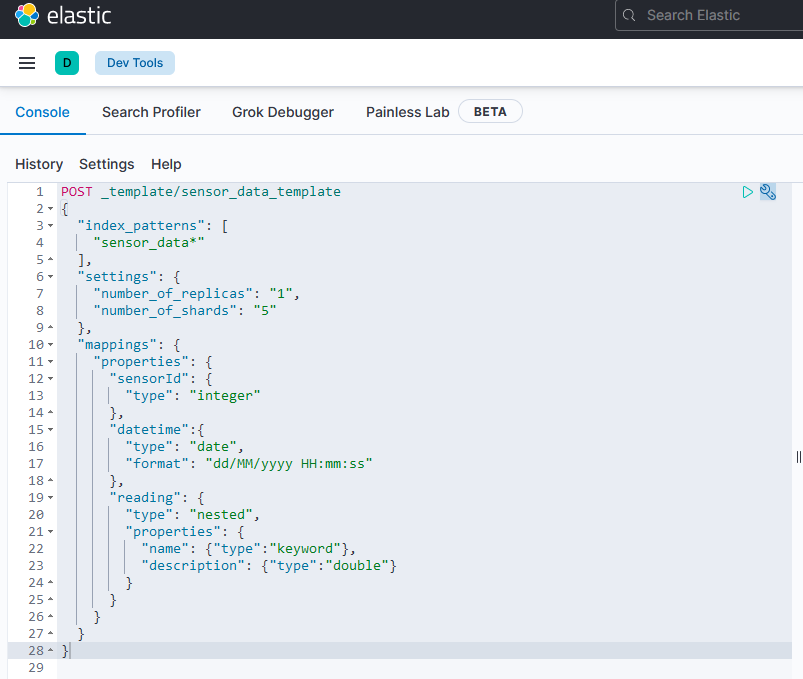
\includegraphics[width=1.1\textwidth]{img/img_crear_patron.png}
	\caption{Crear un índice}
	\label{img_index_pattern}
\end{figure}
\newpage

Una vez creado el índice todos los datos procedentes de losgstash se almacenarán con ese índice permitiendo, dentro del menú Stack Management en el apartado index Managment consultar los datos que va recibiendo.

\begin{figure}[h]
	\centering
	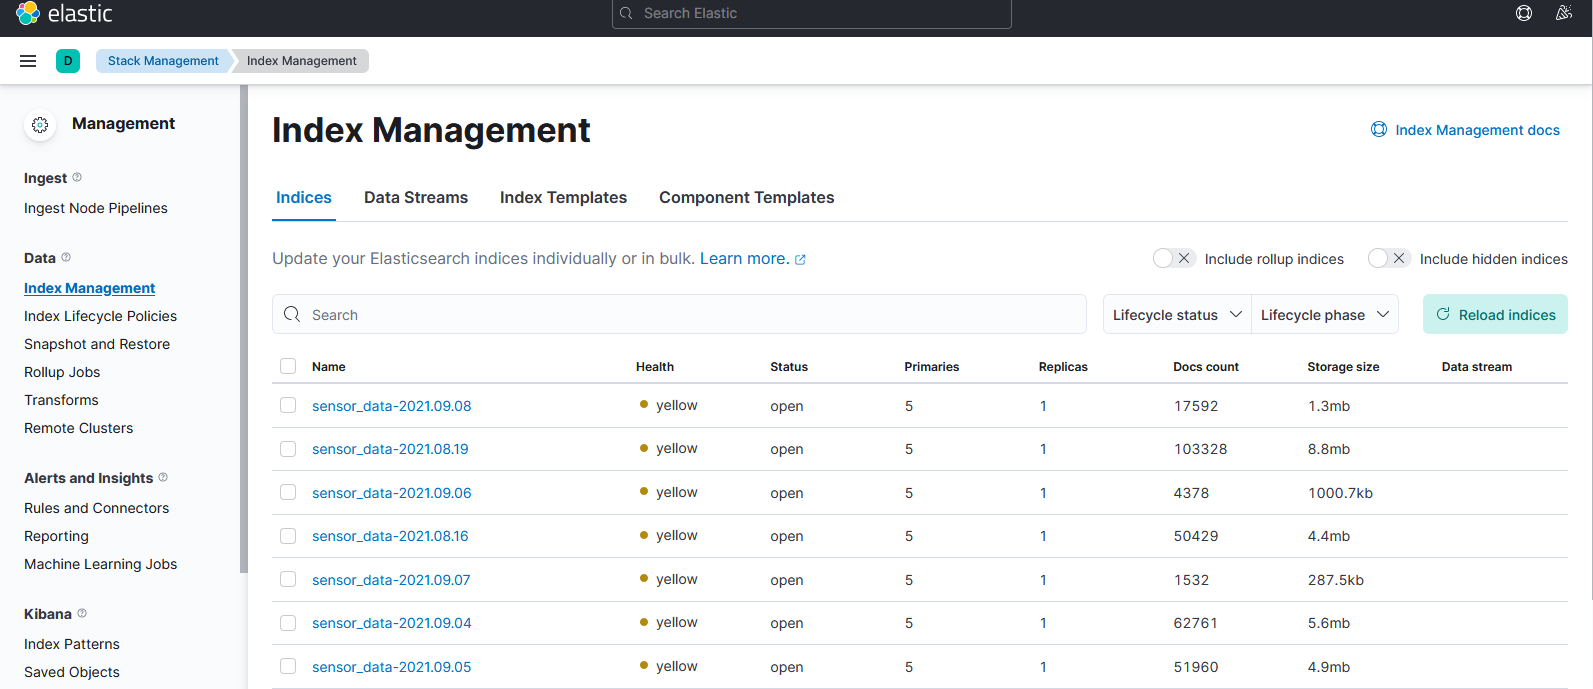
\includegraphics[width=1.1\textwidth]{img/img_index_manager.png}
	\caption{Index Managment}
	\label{img_index_manager.png}
\end{figure}

Para finalizar y poder explorar y visualizar los datos en Kibana es necesarios que exista un ``index pattern'' que diga a Elasticsearch que índices contienen los datos así como especificar de que tipo son, en este caso se ha de crear uno para que albergue todo los datos procedentes de sensores ``sensor\_data-*''\cite{pagina:elastic}

\begin{figure}[h]
	\centering
	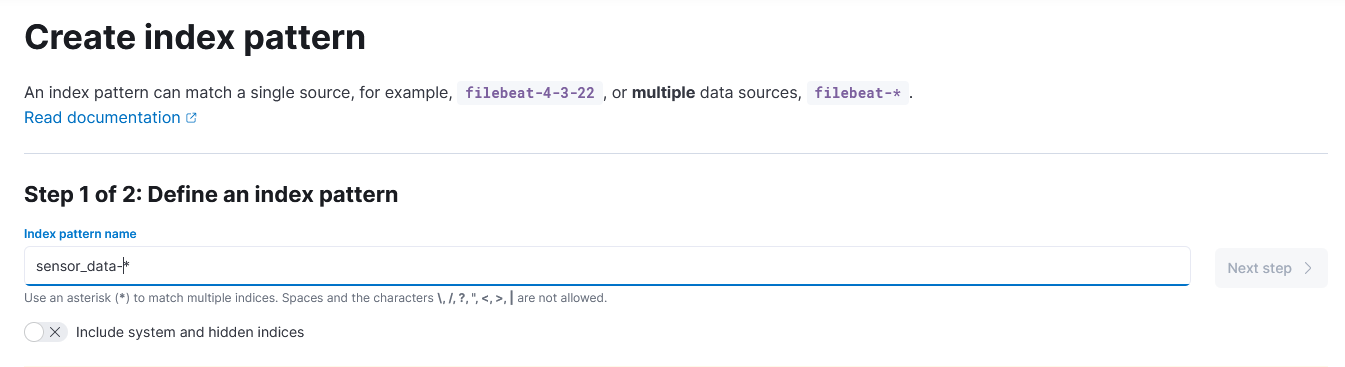
\includegraphics[width=1.1\textwidth]{img/img_create_index_pattern.png}
	\caption{Creación de un index pattern}
	\label{img_create_index_pattern.png}
\end{figure}

Una vez creado el patrón nos pedirá que lo configuremos a nuestro gusto, podremos especificar cuál va a ser el índice de nuestros datos, si el tiempo en el que es indexado a en Elasticsearch ``@timestamp'' u otro campo fecha que nosotros prefiramos.

También se puede cambiar el tipo de cualquier otro campo.

\begin{figure}[h]
	\centering
	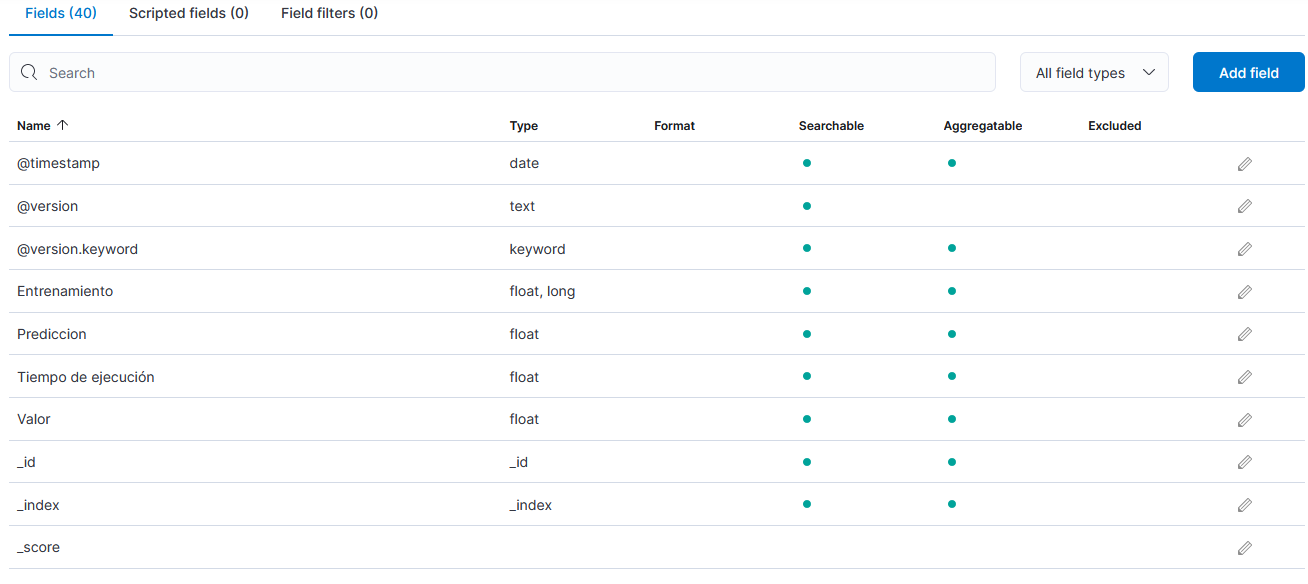
\includegraphics[width=1.1\textwidth]{img/img_conf_index_pattern.png}
	\caption{Configuración de un index pattern}
	\label{img_conf_index_pattern.png}
\end{figure}
\newpage



\subsection{Inicializar \nombrePrograma}

Una vez instalado y configurado ya podremos iniciar nuestro programa introduciendo el siguiente comando como usuario administrador.
\begin{lstlisting}[frame=single]  
systemctl start Monitorizacion_IOT
\end{lstlisting}

También puede ser de utilidad comprobar tanto el estado de nuestro programa como el de Elasticsearch, kibana o logstash en caso de que se haya producido algún fallo.

\begin{lstlisting}[frame=single]  
systemctl status Monitorizacion_IOT

systemctl status elasticsearh
systemctl status kibana
systemctl status logstash
\end{lstlisting}

Si resulta que alguno de los componentes no se encuentra activos podemos reiniciar el servicio.

\begin{lstlisting}[frame=single]  
systemctl restart Monitorizacion_IOT

systemctl restart elasticsearh
systemctl restart kibana
systemctl restart logstash
\end{lstlisting}

\section{Pruebas del sistema}

\subsection{Pruebas de regresión}

A la hora realizar predicciones es extremadamente importante saber cómo de fiable es el modelo que se está utilizando por lo que realizar pruebas es completamente necesario.


\subsubsection{Datasets}
Debido a que no se posee históricos de los datos de los sensores y ya que PRTG sólo recopila datos cuando está conectado en un equipo en funcionamiento, los datasets empleados para realizar las pruebas no son lo suficientemente extensos cómo para entrenar el modelo y que saque predicciones fidedignas. 

Por ello, se realizarán las pruebas con datos recogidos en intervalos de varias de horas y se comprobará cómo se comporta el algoritmo a corto plazo.

Para estas pruebas se usarán dos de los sensores, el que mide la presión de la tubería de agua y el que mide el consumo de la bomba de agua.

\begin{figure}[h]
	\centering
	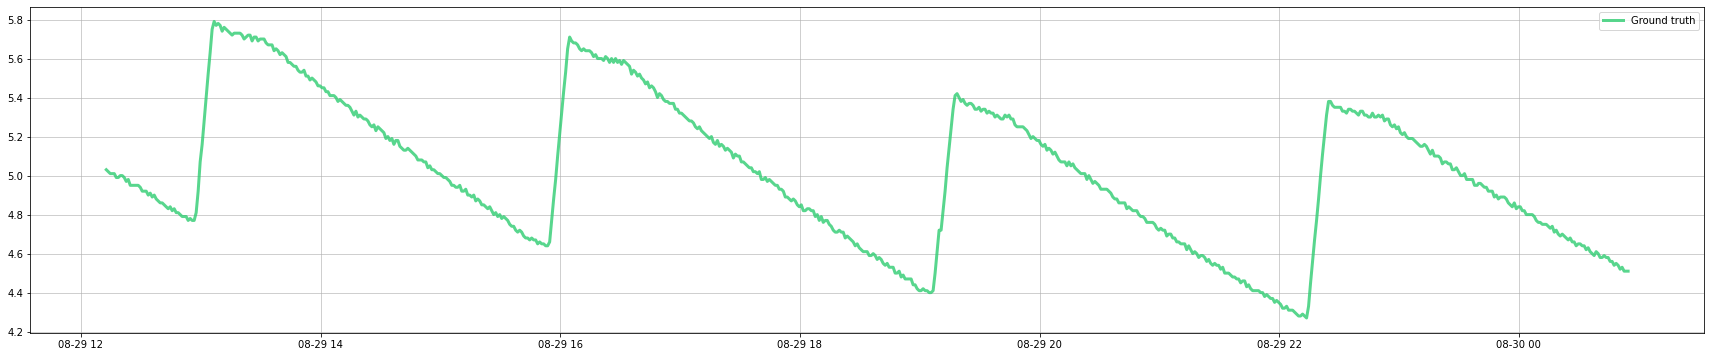
\includegraphics[width=1.1\textwidth]{img/img_dataset2051.png}
	\caption{Dataset sensor de Presión Tubería de Agua}
	\label{img_prediccion_sensor2051}
\end{figure}

\begin{figure}[h]
	\centering
	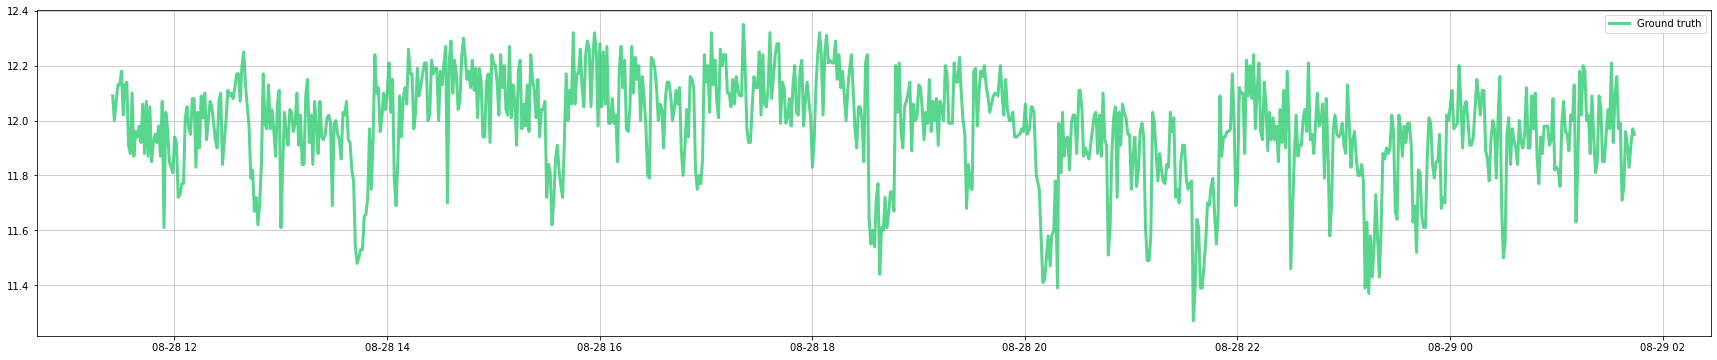
\includegraphics[width=1.1\textwidth]{img/img_2052_trues.png}
	\caption{Dataset sensor Consumo de bomba de agua}
	\label{img_prediccion_sensor2051}
\end{figure}

\subsubsection{Métricas de regresión}

Las métricas de regresión dan un promedio de cuanto de acertadas están las predicciones obtenidas sobre el valor real. Para ello se utilizarán las siguientes métricas:

\subsubsubsection{\textbf{MSE}}

Mean Squared Error o MSE es una de las métricas más comunes en la evaluación de regresión. Mide el error cuadrado promedio de las predicciones.

Se calcula como el promedio de las diferencias al cuadrado entre los valores reales y los predichos.

\begin{equation*}
    MSE = \frac{1}{N} \cdot \sum_{i=1}^{N}(y_i - \hat{y}_i)^2
\end{equation*}

Al elevarse al cuadrado tiende a inflar errores grandes, por lo que cuanto mayor sea la diferencia entre la predicción y los valores reales mayor será el error.

\subsubsubsection{\textbf{RMSE}}

Root Mean Squared Error o RMSE es una extensión de MSE. Esta métrica calcula la raíz cuadrada de MSE, haciendo que las unidades de las métricas sean las mismas que las unidades de los valores originales.

\begin{equation*}
    RMSE = \sqrt{\frac{1}{N} \cdot \sum_{i=1}^{N}(y_i - \hat{y}_i)^2} 
\end{equation*}

Al elevar el MSE al cuadrado se deja de penalizar los errores grandes,

\subsubsubsection{\textbf{MAE}}

Mean Absolute Error o MAE al igual que RMSE las unidades de error coinciden con las unidades de los valores reales y predichos.

MAE no da más o menos peso a los diferentes tipos de error y las puntuaciones aumentan linealmente con el aumento del error.

Se calcula como el promedio del valor absoluto de la diferencia entre los valores reales y predichos.

\begin{equation*}
    MAE = \frac{1}{N} \cdot \sum_{i=1}^{N}|y_i - \hat{y}_i| 
\end{equation*}

\subsubsubsection{\textbf{R2}}

R2 es una métrica que calcula la bondad del modelo.

El mejor valor posible es 1, indicando una predicción perfecta y puede tomar valores negativos si la predicción es muy mala. 
\begin{equation*}
    R^2 = 1 - \frac{\sum(Y_i - \hat{y}_i)^2}{\sum(Y_i - \bar{y}_i)^2}
\end{equation*}


Para los siguientes test se utilizará el modelo SNARIMAX. Se realizan las pruebas con datos 
recopilados de siete días distintos, 
\subsubsection{Pruebas Sensor Consumo Bomba Agua}

\begin{figure}[h]
	\centering
	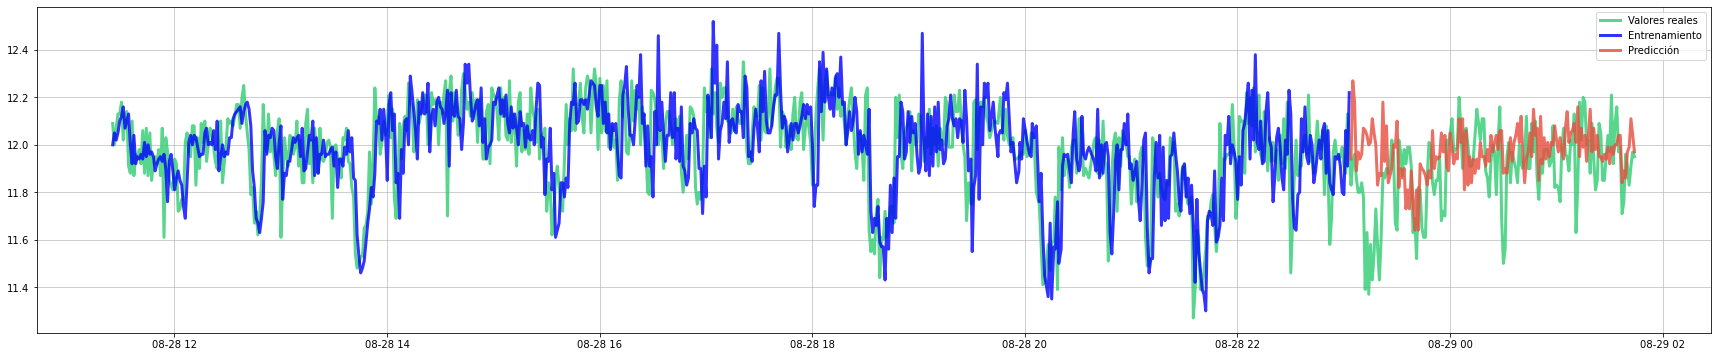
\includegraphics[width=1.1\textwidth]{img/img_2052_1.png}
	\caption{Consumo Bomba Agua en las fechas: 28/08/2021 - 29/08/2021}
	\label{img_prediccion_sensor2051}
\end{figure}

\begin{figure}[h]
	\centering
	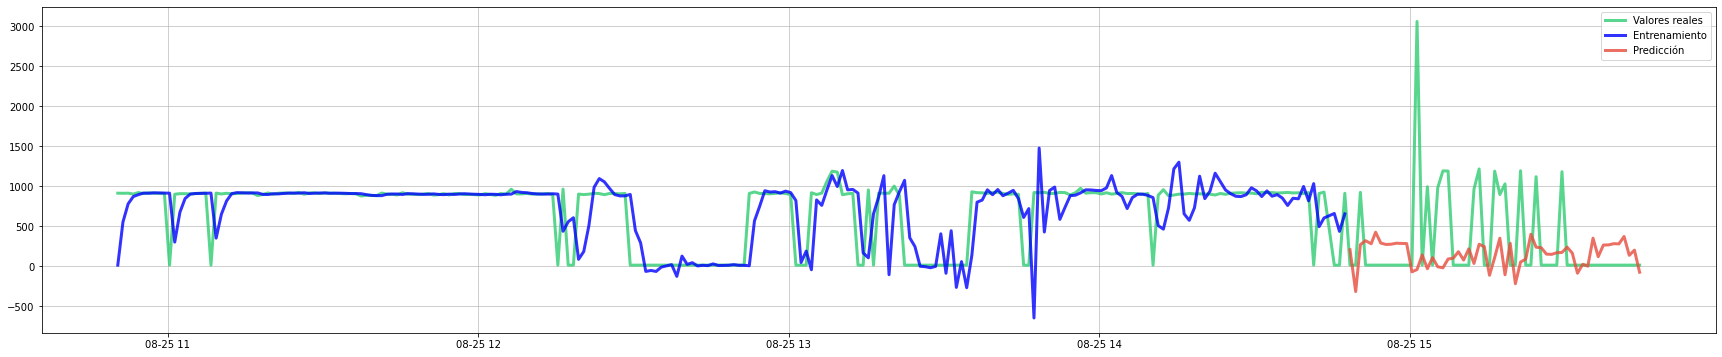
\includegraphics[width=1.1\textwidth]{img/img_2052_4.png}
	\caption{Consumo Bomba Agua en las fechas: 25/08/2021 - 26/08/2021}
	\label{img_prediccion_sensor2051}
\end{figure}

\begin{figure}[h]
	\centering
	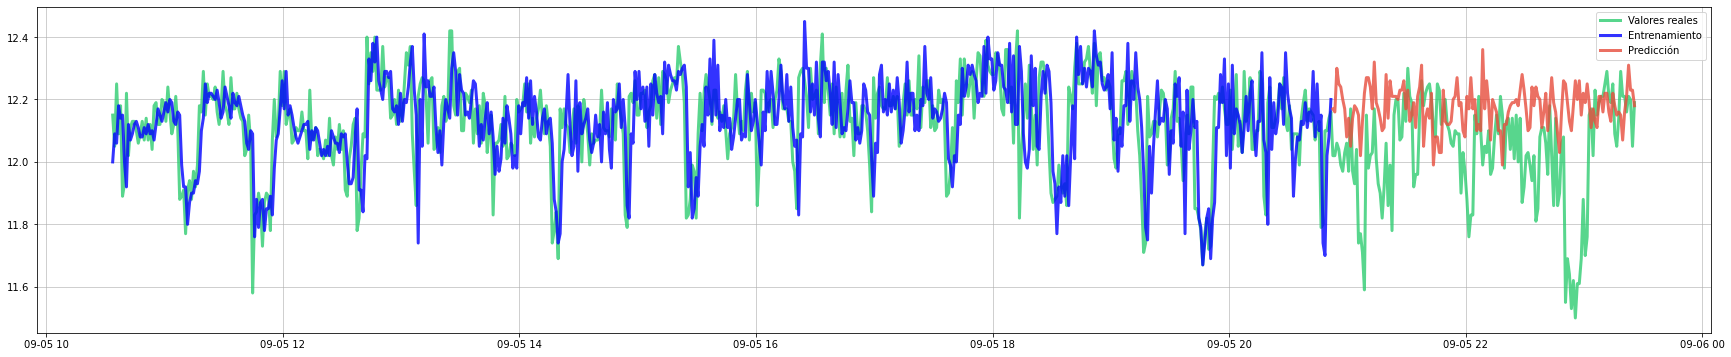
\includegraphics[width=1.1\textwidth]{img/img_2052_5.png}
	\caption{Consumo Bomba Agua en las fechas: 05/09/2021 - 06/09/2021}
	\label{img_prediccion_sensor2051}
\end{figure}

\tablaSmall{métricas Consumo Bomba Agua}{l c c c c}{métricas}
{ \multicolumn{1}{l}{Rango de fechas} & MSE & RMSE & MAE & R2 \\}{ 
05/09/2021 - 06/09/2021 & 0.056 & 0.237     & 0.176     & -0.891\\
28/08/2021 - 29/08/2021 & 0.04 & 0.2        & 0.153     & -0.417\\
27/08/2021 - 28/08/2021 & 0.068 & 0.261     & 0.186     & -0.474\\
25/08/2021 - 26/08/2021 & 431303.37 & 656.737 & 428.61 & -0.272\\
31/07/2021 - 01/08/2021 & 0.035 & 0.188     & 0.142     & -1.125\\
24/07/2021 - 24/07/2021 & 0.019 & 0.137     & 0.111     & -0.439\\\hline

\textbf{Media}          & \textbf{61614.798} & \textbf{93.965} & \textbf{61.436} & \textbf{-0.516}\\
} 
\newpage

\subsubsection{Pruebas Sensor Presión tubería de agua}

\begin{figure}[h]
	\centering
	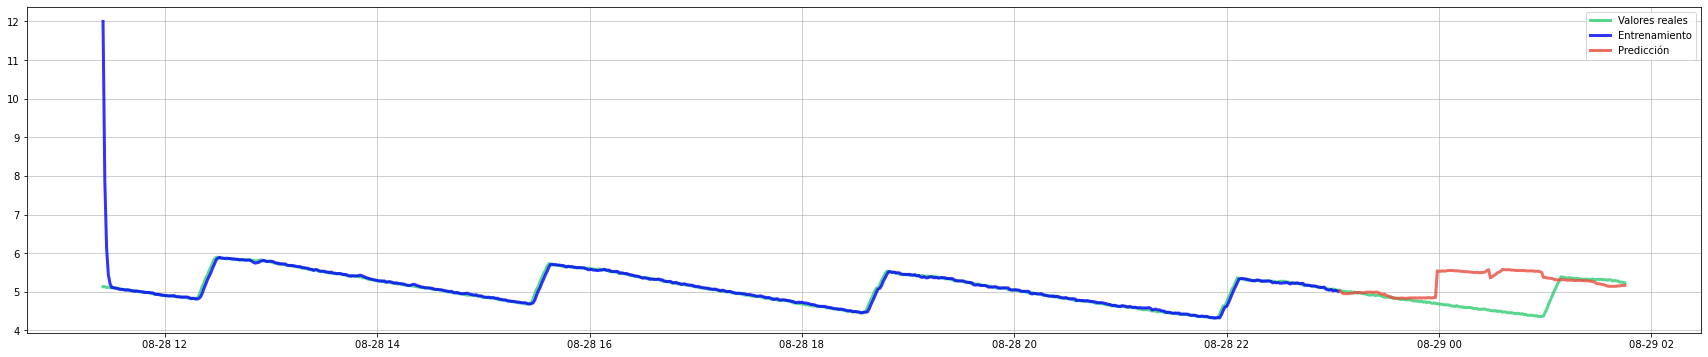
\includegraphics[width=1.1\textwidth]{img/img_2051_2.png}
	\caption{Presión tubería de agua en las fechas: 28/08/2021 - 29/08/2021}
	\label{img_prediccion_sensor2051}
\end{figure}

\begin{figure}[h]
	\centering
	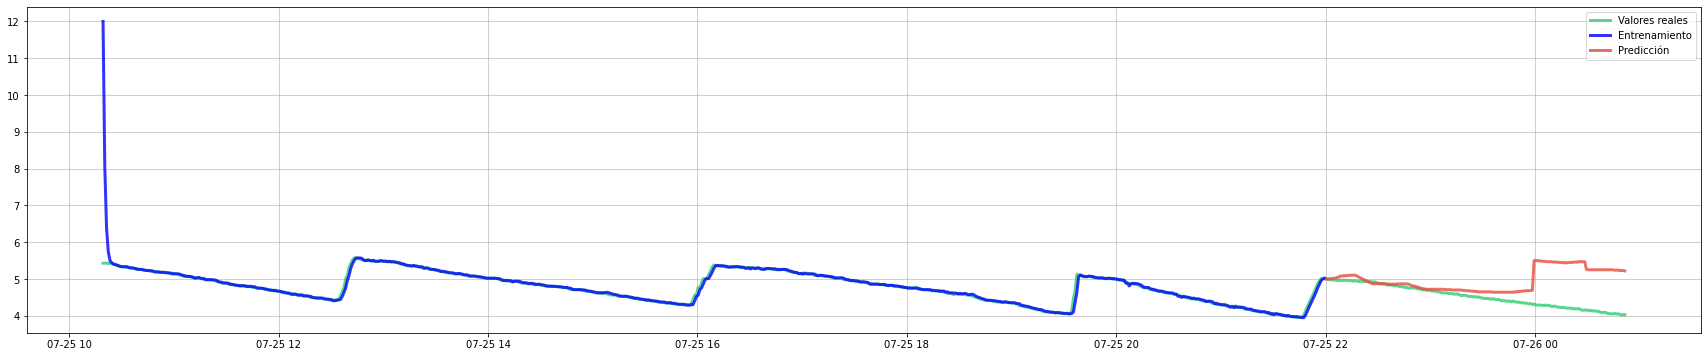
\includegraphics[width=1.1\textwidth]{img/img_2051_6.png}
	\caption{Presión tubería de agua en las fechas: 25/07/2021 - 26/07/2021}
	\label{img_prediccion_sensor2051}
\end{figure}

\begin{figure}[h]
	\centering
	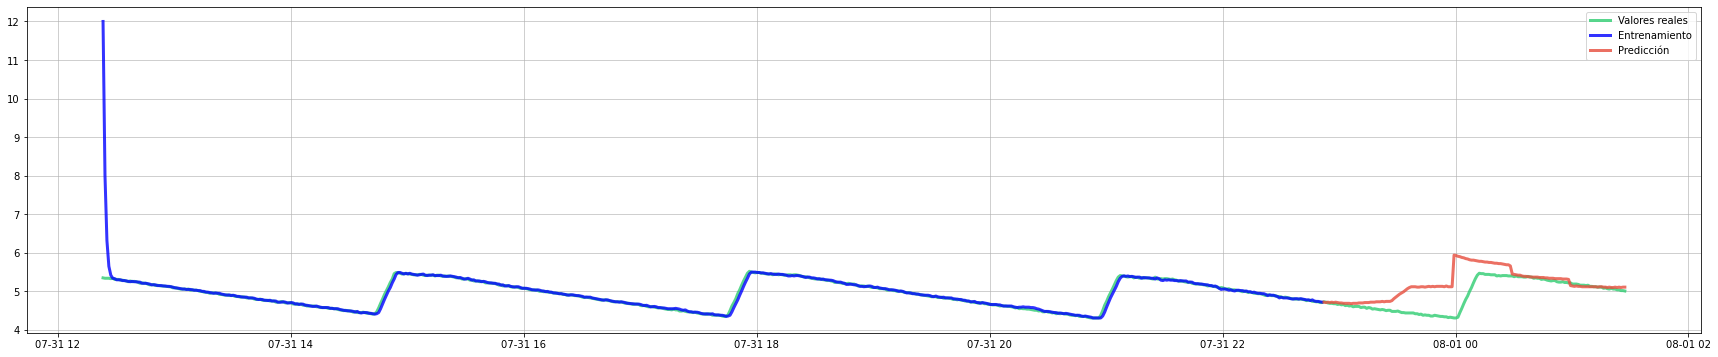
\includegraphics[width=1.1\textwidth]{img/img_2051_7.png}
	\caption{Presión tubería de agua en las fechas: 31/07/2021 - 01/08/2021}
	\label{img_prediccion_sensor2051}
\end{figure}
\newpage

\tablaSmall{métricas Presión tubería de agua}{l c c c c}{métricas}
{ \multicolumn{1}{l}{Rango de fechas} & MSE & RMSE & MAE & R2 \\}{ 

08/09/2021 - 09/09/2021 & 0.125 & 0.354 & 0.322 & -0.217\\
29/08/2021 - 30/08/2021 & 0.193 & 0.44 & 0.358 & -1.658\\
28/08/2021 - 29/08/2021 & 0.404 & 0.635 & 0.441 & -2.936\\
25/08/2021 - 26/08/2021 & 0.159 & 0.399 & 0.358 & -0.187\\
31/07/2021 - 01/08/2021 & 0.218 & 0.467 & 0.298 & -0.381\\
25/07/2021 - 26/07/2021 & 0.461 & 0.679 & 0.453 & -4.156\\\hline
\textbf{Media}          & \textbf{0.222} & \textbf{0.424} & \textbf{0.318} & \textbf{-1.362}\\
} 
\begin{comment}


\begin{figure}[h]
	\centering
	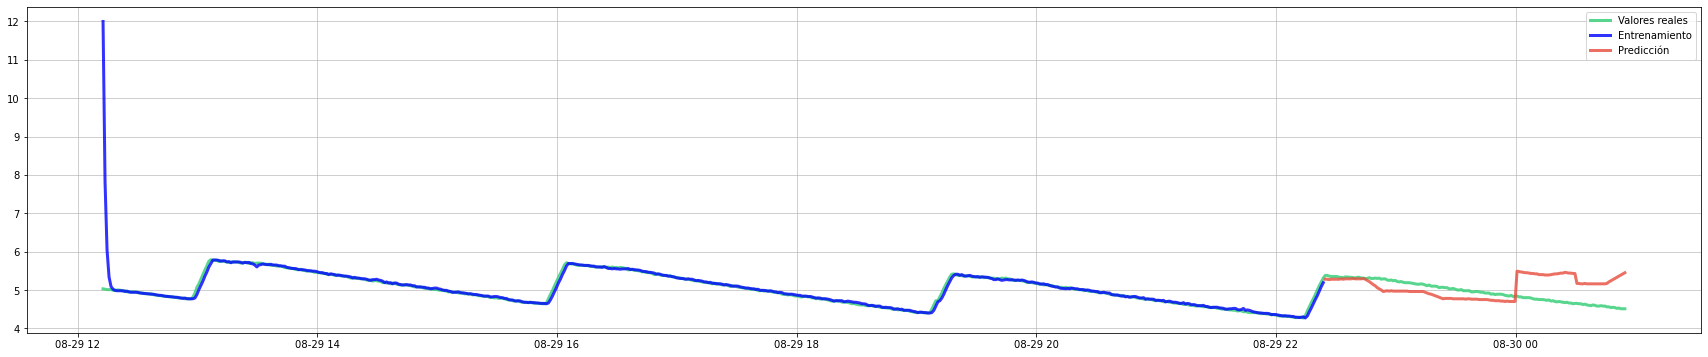
\includegraphics[width=1.1\textwidth]{img/img_pred_2051.png}
	\caption{predicción con modelo SNARIMAX sensor de Presión tubería de agua}
	\label{img_prediccion_sensor2051}
\end{figure}

\begin{figure}[h]
	\centering
	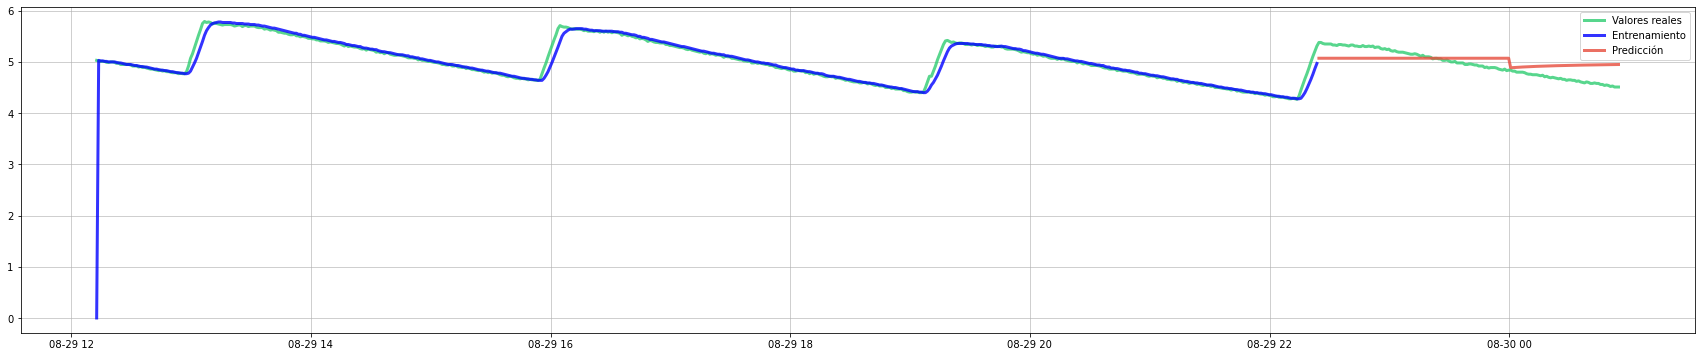
\includegraphics[width=1.1\textwidth]{img/img_predDETRENDER_2051.png}
	\caption{predicción con modelo Detrender sensor de Presión tubería de agua}
	\label{img_prediccion_sensor2051}
\end{figure}

\tablaSmall{métricas Presión tuberñia de agua 1}{l c c c c}{métricas}
{ \multicolumn{1}{l}{Modelos} & MSE & RMSE & MAE & R2 \\}{ 
SNARIMAX & 0.193 & 0.439 & 0.358 & -1.658\\
Detrender & 0.05 & 0.224 & 0.197 & 0.305\\

} 

\end{comment}
